% TEMPLATE for Usenix papers, specifically to meet requirements of
%  USENIX '05
% originally a template for producing IEEE-format articles using LaTeX.
%   written by Matthew Ward, CS Department, Worcester Polytechnic Institute.
% adapted by David Beazley for his excellent SWIG paper in Proceedings,
%   Tcl 96
% turned into a smartass generic template by De Clarke, with thanks to
%   both the above pioneers
% use at your own risk.  Complaints to /dev/null.
% make it two column with no page numbering, default is 10 point

% Munged by Fred Douglis <douglis@research.att.com> 10/97 to separate
% the .sty file from the LaTeX source template, so that people can
% more easily include the .sty file into an existing document.  Also
% changed to more closely follow the style guidelines as represented
% by the Word sample file. 

% Note that since 2010, USENIX does not require endnotes. If you want
% foot of page notes, don't include the endnotes package in the 
% usepackage command, below.

% This version uses the latex2e styles, not the very ancient 2.09 stuff.

% Updated July 2018: Text block size changed from 6.5" to 7"

\documentclass[letterpaper,twocolumn,10pt]{article}
\usepackage{usenix2019,epsfig,endnotes}

\usepackage{pgfplots}
\pgfplotsset{compat=newest}
\usepackage{footnote}
\makesavenoteenv{tabular}


\begin{document}

%don't want date printed
\date{}

%make title bold and 14 pt font (Latex default is non-bold, 16 pt)
\title{\Large \bf 9Back : Making Our Plans Great Again}

%for single author (just remove % characters)
\author{
{\rm Maxwell Bland}
\and
{\rm Leon Cheung}\\ \\
University of California, San Diego
\and
{\rm Kilian Pfeiffer}\\
% copy the following lines to add more authors
% \and
% {\rm Name}\\
%Name Institution
} % end author

\maketitle

% Use the following at camera-ready time to suppress page numbers.
% Comment it out when you first submit the paper for review.
\thispagestyle{empty}


\subsection*{Abstract}
The following paper describes a set of benchmarks run on the Plan 9 operating system. In particular, it uses the only actively developed branch, 9FRONT "RUN FROM ZONE!" (2018.09.09.0 Release). The goal of this project is to provide researchers and enthusiasts with greater insight into the current state of the operating system's performance and capabilities of interaction with hardware. Through tests of CPU, Memory, Network, and File System operations, we will gain insight on bottlenecks in the system's performance and the interactions between low-level (hardware) and high-level (OS) system components. These performance statistics will be contrasted with subjective experiences of ``responsiveness''.

\section{Introduction}

Plan 9 from Bell labs is a distributed operating system which emerged around the 1980's. It built upon the ideas of UNIX, but adopted an ideology that ``everything is a file''. Although the system was marketed in the 90's, it did not catch on, as prior operating systems had already gained enough of a foothold. Eventually, during the 2000's, Bell Labs ceased development on Plan 9, meaning official development halted. Unofficial\footnote{This is debatable. If you adopt an orphan, are they not your official child?} development continues on the 9front fork of the codebase, with new support for Wi-Fi, Audio, and everything anyone could ever want or need. 

The experiments were performed as a group using a shared codebase and a single machine described in the following section. The measurements were performed via programs written in Plan 9's \textit{special} version of C 99. The compiler used were the x86 versions of Plan 9's C compiler, 8c. The compiler was run with optimizations disabled. Version numbers are not available. Measurements were performed on a single machine running Plan 9 directly from hardware; given the nature of the Plan 9 system,
additional metrics could be established for networked file systems and CPU servers; these measurements were not done for sake of simplicity, and because results under these conditions should be inferrable from the results cataloged within this paper plus network overheads. 

The use of actual hardware for this task should have less variance compared to measurements performed within a VM, although there were several points in time where it became clear that Plan 9 was not neccessarily able to handle the hardware interface as expected, such as during the high contention disk access task, which caused I/O errors to shoot off from the SSD.

The project was accomplished over the course of ten weeks in short five to twenty hour bursts, wherein team members took turns on implementation tasks according to their respective amounts of free time. In total, due to difficulties inherent with the particular operating system chosen for benchmarking, each team member spent around 30 to 40 hours on this project. 

Benchmarking a forty year old bunny-focused OS maintained by less than 10 strangers including us and making it jump through rings of fire was admittedly a weird flex but okay. 

\section{Machine Description}

We ran this beautiful operating system of the gods on a Thinkpad T420, the machine of true developers.

{\tt \small
\begin{verbatim}
    Processor: model, cycle time, cache sizes (L1, L2,
      instruction, data, etc.)
      Intel(R) Core(TM) i5-2520M CPU @ 2.50GHz (Sandy Bridge)
      cache size 3072 KB
      L1$	128 KiB	
        L1I$	64 KiB	2x32 KiB	8-way set associative	 
        L1D$	64 KiB	2x32 KiB	8-way set associative	write-back
      L2$	512 KiB 2x256 KiB	8-way set associative	write-back
      L3$	3 MiB   2x1.5 MiB	12-way set associative	write-back
      cpu family 6
      model 42
      stepping 7
      siblings 4
      cores 2
      fpu yes
      fpu_exception yes
      fpu_exception yes
      bogomips 4986.98
      clflush size 64
      cache_alignment 64
    Details at https://en.wikichip.org/wiki/
    intel/core_i5/i5-520m 

    Memory bus
      DDR3-1333
      i/o-bus-frequency: 666MHz
      bus-bandwith:  10656 MB/s
      memory-clock:  166MHz
      Column Access Strobe (CAS) latency:

    I/O bus
      SataIII-speed: 600MB/s

    RAM size
      8 GB
    Disk: capacity, RPM, controller cache size
      Samsung SSD 860 EVO 500GB
      Capacity: 500GiB
      RPM: 550MB/s read, 520 MB/s write
       and 98,000 IOPS (Read QD32)
      Controller Cache Size: 512MB 
    Network card speed:
     Intel 82579 LM Gigabyte: 1Gb/s
     intel Centrino Ultimate-N 6300: 450 Mbps
      
    Operating system (including version/release) 
      9FRONT "RUN FROM ZONE!" (2018.09.09.0 Release)
\end{verbatim}
}

\section{Experiments}

For each section, we report the base hardware performance, make a guess as to how much overhead software will add to base hardware performance, combine these two into an overall prediction of performance, and then implment and perform the measurement. In all cases, we run the experiment multiple times, and calculate the standard deviation across measurements. We use the \texttt{cycles()} syscall to record the timestamp. Dynamic CPU frequency scaling was disabled for all trials, and all trials were restricted to a single core.

\subsection{Measurement Overhead (Reading Time)}

The following section reports overheads of reading time. One trial involves looping over 16 \texttt{cycles} timing calls, $2^{16}$ times. We average out for each call of \texttt{cycles}, and we do 64 trials altogether.

Since we imagine getting the current cycles clock is a fast operation, so we
estimate the hardware performance to be on the scale of nanoseconds, since one
clock cycle takes approximately 0.5 nanoseconds. We think that the
\texttt{cycles} call should do something similar to reading from the cycle
counter, so it should be almost instantaneos, perhaps on the order of 2ns.
[Page 547 of https://www.intel.com/content/dam/www/public/us/en/documents/manuals/64-ia-32-architectures-software-developer-vol-2b-manual.pdf]

The software cost of this should be low to non-existent, since that value is 
directly loaded into two registers, which might be directly examined under normal 
circumstances. It is the case that Plan 9's C compiler does not accept assembly directives, 
and thus we were forced to use the \texttt{cycles} call, which may be doing extra work.

This would put our predicted cost at around 2 to 10 nanoseconds, accounting for potential
variations due to operating system tasks such as context switching, interrupts, and 
other architectural lags.

Our results are shown in table 1; it seems we may have underestimateed the cost of hardware 
and software in measurement of time. We feel that our methodology, however, is sound, given the
incredibly low degree of variability in our results. Units are reported in nanoseconds.

\subsection{Measurement Overhead (Loop Overhead)}

In order to measure the loop overhead, we took the time at the end of a loop
iteration and at the start of a loop iteration, and find the difference between
those to measure the loop overhead time. We repreat this 16384 times within
each trial, and perform 64 trials. We average over all of these trials.

The cost of doing a single for loop based branch in hardware is also very low.
Assuming a compare, jump, and register increment take 3 to 5 cycles, and adding
additional overheads for branch misprediction, the loop overhead should be around
10 cycles. 
[Patterson, David A.; Hennessy, John L. Computer Organization and Design: The Hardware/Software Interface.]

Software, will slow this down due to random interruptions while executing, as mentioned before.
Other system processes may need the processor, and thus the latency might be roughly twice 
this.

As a prediction, the cost of a loop will be on the order of 20 nanoseconds, maybe less, since
our hardware estimate may be a bit too lenient.

The results for this experiment are also in table 1; we did underestimate the cost of a loop by a bit;
we feel this is most likely due to higher hardware costs than expected, perhaps due to the ineffiencies
of the processor's branch predictor or just high cycle count instructions. We have every reason to believe our methodology was sound.

\begin{figure}
	\centering
    \begin{tabular}{lll}
      & Reading (ns) & Loop (ns) \\
Hardware Guess  & 1 & 5\\
Software Multiplier & 2-10 & 2 \\
Prediction & 2-10 & 10\\
Average  & 11 & 17.2 \\
Std Dev. & 0 & 0
\end{tabular}
\caption{Measurement Overheads}
\label{tab:generaloverheads}
\end{figure}


\subsection{Procedure Call Overhead}

In measuring the function overhead, we created functions of zero to seven integer arguments,
we then proceeded to call eacah of these functions 20000 times, and found the average time taken over these 20000 calls. Overall, increment overhead was almost non-existent.

The hardware cost of a procedure call using the standard c calling convention should not be that high, as it is almost all done in registers. The caller pushes the arguments to the stack (very little cost), saves the return address, the frame pointer, and calls the function. There is also all the take-down cost for the function call, and the jumping of the instruction pointer, which will clear the incoming buffer of instructions. The hardware cost of this should be significant but not insane; we
are thinking on the order of 30 cycles, so around 15 or less nsec.
[https://9p.io/sys/doc/compiler.html]

The software cost of a function call in plan 9 is remarkably small, as the compiler stores all argument positions relative to a stack pointer, and thus needs to consider only one piece of metadata while making a call. There is still the threat of context switches, so the software cost may be a multiplier between 1 and 2.

This puts our prediction for the cost to be somewhere around 15 to 20 nanoseconds for a function call, independent of the number of parameters passed.

Our results are recorded in table 2; we were roughly in line with our estimates, though there is a significant degree of variance in the results, most likely due to needing to make a reference back into DRAM or context switches. This was a straightforward quantity to measure and most likely our results are accurate. 

As a final note, there is little overhead for adding arguments to a function call in plan nine, most likely due to the stack pointer relative addressing and our lack of tests for access times to the arguments vs other operating systems.

\begin{figure}
	\centering
\begin{tabular}{lll}
Hardware Guess       & 15 nsec & \\
Software Multiplier Guess       & 1-2 &  \\
Prediction       & 17 nsec &  \\
    Num Args & Average (nsec)   & Std Dev. (nsec)  \\
0& 14.487840& 8.702724
1& 14.892560& 8.991838
2& 15.215200& 9.187626
3& 14.844640& 8.996905
4& 14.883760& 8.986072
5& 15.223920& 9.204537
6& 14.851200& 8.963965
7& 15.226480& 9.198042
8& 15.264640& 9.227006
\end{tabular}
\caption{Procedure Call Overheads}
\label{tab:proccalloverheads}
\end{figure}

\subsection{System Call Overhead}

To measure the syscall overhead, we used the \texttt{errstr(2)} syscall, in
particular, \texttt{rerrstr(char*, vlong)}. \texttt{reerrstr} reads the error
string for the error of a previous syscall, and does not clear the errstr
buffer. Within each trial, we performed the syscall 16384 times, and averaged
over 64 trials.

Data from IBM puts the cost of making a system call on the Pentium processor in 1997/1995
to be 223 cycles, or roughly 1.68 usec for that processor. Our processor is much faster,
putting the timing at around 100 nsec.
%[https://www.ibm.com/developerworks/ community/blogs/kevgrig/entry /approximate_overhead_of_system_ calls9?lang=en]

It is likely that the overhead of a syscall beyond this is pretty high due to
the actual operations and implementation of the syscall operation. Thus, the
cost could be 10x the hardware cost.

That puts our estimate at around 1000 nsec or 1usec, which still seems reasonable for a system call.

Results are shown in table three and reveal a slight overestimate on our part, though perhaps not an 
unreasonable one. Notably, this cost is much, much higher than a empty-body procedure call. We do not
have any reason to believe that Plan 9 would be caching the results of this system call so that subsequent
calls do not need to trap to the OS. This may be a potential source of optimizations.

Our methodology for evaluating this experiment was straight forward enough and is likely correct.

\begin{figure}
	\centering
    \begin{tabular}{ll}
            & System Call Overhead \\
    Hardware Guess  & 100 nsec  \\
    Software Multiplier  & 10x \\  
    Prediction  & 1000 nsec \\
    Average  & 861 nsec\\
    Std Dev. & 70.8 nsec          
    \end{tabular}
\caption{Syscall Overhead}
\label{tab:syscalloverheads}
\end{figure}

\subsection{Task Creation Time}

We measured process creation overhead in two different ways, one in which we
\texttt{rfork}'ed a new process without copying the parent state to the child,
and, \texttt{fork}, where the child will copy all of the parent's file
descriptors, and share the other state as normal. We do these 20000 times for
each type of \texttt{fork} and we average over all of these calls. This methodology
results from the fact that Plan 9 does not have kernel threads.

The hardware costs of a light fork should be much less than a heavy fork, since
resources do not need to be shared, but because our processes are minimal, it
is likely this difference is negligible. Plan 9 adopts a very similar memory management
scheme to Unix, and so fork semantics are roughly equivalent, including copy-on-write. (The 
following citation contains a breakdown of almost every line in the Plan 9 kernel source code).
[http://citeseerx.ist.psu.edu/viewdoc/download?doi=10.1.1.75.5409&rep=rep1&type=pdf]. The number
of cycles involved in forking a process is likely huge, however, and in the tens of thousands of 
cycles, since all sorts of meta data (such as the page table) needs to be copied over. There 
aren't many good resources online which have benchmarked the number of cycles involved in a fork.

Since the software overhead of a fork is the fork itself, the hardware and software costs are 
pretty much interlinked in this particular experiment. Thus, we ignore a software multiplier, setting it
equal to 1. 

That puts our estimate at around 60,000 cycles or 30,000 nsec for both fork operations. We do not 
believe that Plan 9's lightweight fork operation will help much, and that most of the resources 
and state will still need to be copied to the child.

Our results are recorded in table 4; we were roughly in line with our estimates, but there is something quite interesting going on with Plan 9's heavy fork, the equivalent of running a process vs. a kernel thread. There is no difference in average fork time, but there is a huge variation in the two. Heavy forks have a long tail; in future work, it may be interesting to plot this long tail, and analyze the impact it has on end-user applications.

In general, programmers should opt for light forks, if possible. Just don't bend them!

\begin{figure}
	\centering
\begin{tabular}{lll}
        & Light Fork & Heavy Fork \\
Hardware Guess & 30 usec & 30 usec \\
Software Multiplier & 1x & 1x \\
Prediction & 30 usec & 30 usec \\
Average & 27.250  usec & 28.674  usec \\
Std Dev & 1.83 usec & 58.068 usec                  
\end{tabular}
\caption{Fork Overheads}
\label{tab:forkoverheads}
\end{figure}

\subsection{Context Switch Time}

Finally, to measure context switching, we created a pipe in a parent process,
and forked off a new child process. We forced a context switch by writing to
the pipe in the parent and then waiting for the child to read from the pipe
and terminate. We take the time between when the parent goes to sleep and when
the parent wakes up again after the child's termination. Then, we subtract
the overhead of reading from the pipe and closing the pipe (which happens in
the child), and divide the time in half to account for the two context switches.
We repeat this measurement 1000 times and use a new pipe each time. To take
the time of a context switch, we take the minimum time over all of these trials.

We estimated the base hardware cost of context switching while pinned to a single CPU to
be on the order of around 1600 ns based upon benchmarks done on the Intel E5-2620, another
Sandy Bridge processor model. [https://blog.tsunanet.net/2010/11/how-long-does-it-take-to-make-context.html]

Our prediction for the software cost of this is going to be quite large, most likely around 10x, since there
are so many factors involved and our method of triggering a context switch is not the most scientific 
method due to limitations in low-level threading primitives for Plan 9. 

This puts our prediction right around 16 usec; the cost of the context switch itself may be less than 
this in Plan 9, but in order to measure this, we will need to develop modifications to the kernel. 
These modifications are reserved for future work.

The results are included in table 5. Our estimates were a bit too pessimistic, however, they were close 
to the truth, as the results were skewed to values even greater than 16 microseconds. 

In general, our methodology could be improved; a lack of familiarity with such a niche system reduced our ability to benchmark effectively. 

\begin{figure}
	\centering
\begin{tabular}{ll}
Hardware Cost  & 1600 nsec  \\
Software Multiplier  & 10x   \\
Prediction  & 16 usec    \\
Average  & 13.458 usec    \\
Std Dev. & 9.569 usec     \\
Min      & 7.862 usec   
\end{tabular}
\caption{Context Switch Overheads}
\label{tab:conswitchoverheads}
\end{figure}

\subsection{RAM Access Time}

To measure ram access time we allocate a $1.6$ GB array on the heap, and iterated through it with changing stride size to hit L1, L2 cache and finally memory. The stride size gets increased by factor 1.01 for each iteration. Predictions are presented in fig.~\ref{tab:accesstimepred}, while the measurements are presented in fig.~\ref{tab:accesstime}. Figure~\ref{fig:memlatency} presents the plot of the mean in orange and standard deviation in blue with the last index accessed in the iteration on the $x$ axis, and memory access latency is displayed on a logarithmic scale $y$ axis. The measurements are not completely free of overhead, but still a transition from L1 to L2, and from L2 to memory is visible in the graph. 

We estimated the base hardware cost of memory accesses based upon well documented knowledge of the timings of such memory accesses. According to work done on breaking AES, L1 cach is available after 3 cycles, L2 after 11, and memory after this takes hundreds of cycles. [http://palms.ee.princeton.edu/system/files/Cache-timing+attacks+on+AES.pdf]

For measurements like the one outlined above, there is very little software cost involved; thus our software overhead estimate is a multiplier of 1.

As a result, our prediction is that the memory access times under Plan 9 will correspond well with other 
operating systems and personal computers, particularly those running x86 processors.

And our results, shown in tables 6, 7, and figure 8, reveal that our prediction was, indeed, correct. Standard deviations were high for some portions, due to natural variations in experimental conditions. This is an 
important result from a security point of view, as it reveals that Plan 9 may be vulnerable to significant 
timing side channel attacks, something which should be addressed by the community in due time, especially
considering the distributed nature of the Plan 9 system.

Our methodology has revealed a common expectation and typical empirical feature of x86 processors, and 
thus we are confident in our methodology.

\begin{figure}
	\centering
	
	\begin{tabular}{lll}
		prediction L1 latency  & 2-3 cycles & 0.8-1.2 nsec  \\
		prediction L2 latency  & 10 cycles  & 4 nsec \\
		prediction memory latency  & 100 cycles   & 40 nsec \\
	\end{tabular}
	\caption{RAM access time prediction}
	\label{tab:accesstimepred}
\end{figure}

\begin{figure}
	\centering

	\begin{tabular}{ll}
		L1 latency  & 6 nsec  \\
		L2 latency  & 10 nsec  \\
		Memory   & 250 nsec   \\
	\end{tabular}
	\caption{RAM access time measurements}
	\label{tab:accesstime}
\end{figure}

\begin{figure}
	\centering
	% This file was created by matplotlib2tikz v0.6.18.
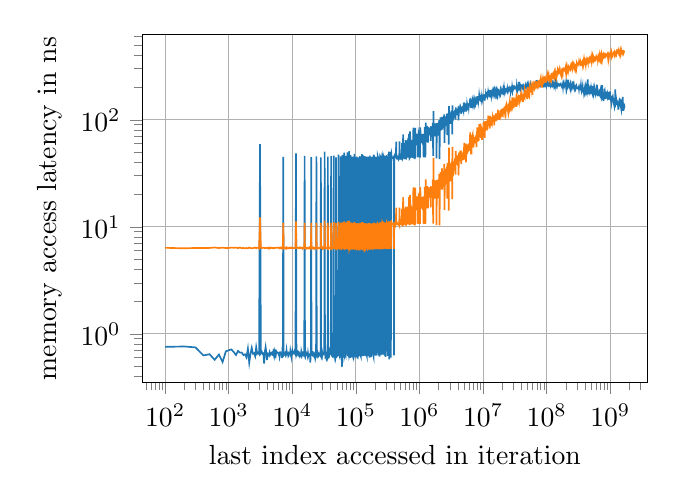
\begin{tikzpicture}

\definecolor{color0}{rgb}{0.12156862745098,0.466666666666667,0.705882352941177}
\definecolor{color1}{rgb}{1,0.498039215686275,0.0549019607843137}

\begin{axis}[
height=6cm,
tick align=outside,
tick pos=left,
width=8cm,
x grid style={white!69.01960784313725!black},
xlabel={last index accessed in iteration},
xmajorgrids,
xmin=43.5293709083906, xmax=3850966979.34791,
xmode=log,
y grid style={white!69.01960784313725!black},
ylabel={memory access latency in ns},
ymajorgrids,
ymin=0.350899005696519, ymax=624.477107437338,
ymode=log
]
\addplot [semithick, color0, forget plot]
table [row sep=\\]{%
100	0.7561587 \\
200	0.7623542 \\
300	0.7475935 \\
400	0.629209 \\
500	0.6456748 \\
600	0.5725871 \\
700	0.6409368 \\
800	0.5454686 \\
900	0.6859854 \\
1000	0.7028513 \\
1100	0.7155418 \\
1200	0.6760355 \\
1300	0.6337066 \\
1400	0.6928203 \\
1500	0.6678323 \\
1600	0.6689813 \\
1700	0.6337192 \\
1800	0.6440373 \\
1900	0.6032446 \\
2000	0.728 \\
2100	0.5365967 \\
2200	0.6541437 \\
2300	0.7415767 \\
2400	0.6532993 \\
2500	0.6599273 \\
2600	0.6183721 \\
2700	0.7501573 \\
2800	0.652184 \\
2900	0.668024 \\
3000	0.648691 \\
3100	59.1957777 \\
3200	0.661864 \\
3300	0.6820674 \\
3400	0.6526132 \\
3500	0.6581793 \\
3600	0.5273936 \\
3700	0.6801882 \\
3800	0.752 \\
3900	0.6661051 \\
4000	0.5682816 \\
4100	0.6557561 \\
4200	0.6494798 \\
4300	0.6304792 \\
4400	0.6726069 \\
4500	0.6426321 \\
4600	0.6621178 \\
4700	0.6671611 \\
4800	0.6382351 \\
4900	0.6351189 \\
5000	0.6770643 \\
5100	0.6409368 \\
5200	0.678575 \\
5300	0.6223954 \\
5400	0.661864 \\
5500	0.6366914 \\
5600	0.6892431 \\
5700	0.6786339 \\
5800	0.6657327 \\
5900	0.6642771 \\
6000	0.6651436 \\
6100	0.6447821 \\
6200	0.6547794 \\
6300	0.6095769 \\
6400	0.6397374 \\
6500	0.6596484 \\
6600	0.6474071 \\
6700	0.6499231 \\
6800	0.64858 \\
6900	0.5955031 \\
7000	0.7549728 \\
7100	0.6623473 \\
7200	45.0235513 \\
7300	0.6291455 \\
7400	0.6356225 \\
7500	0.6431298 \\
7600	0.6589203 \\
7700	0.6652398 \\
7800	0.6456748 \\
7900	0.6298698 \\
8000	0.649566 \\
8100	0.6947115 \\
8200	0.6462198 \\
8300	0.6427939 \\
8400	0.6597454 \\
8500	0.6652398 \\
8600	0.6350307 \\
8700	0.6511528 \\
8800	0.64 \\
8900	0.6613441 \\
9000	0.6619245 \\
9100	0.6459102 \\
9200	0.6439379 \\
9300	0.686743 \\
9400	0.6573158 \\
9500	0.6736646 \\
9600	0.6739021 \\
9700	0.6297174 \\
9800	0.6635179 \\
9900	0.6747918 \\
10000	0.6962758 \\
10200	0.650612 \\
10400	0.6550603 \\
10600	0.6589568 \\
10800	0.683649 \\
11000	0.6508456 \\
11200	0.6384481 \\
11400	48.6467403 \\
11600	0.64005 \\
11800	0.6589568 \\
12000	0.651595 \\
12200	0.6409368 \\
12400	0.6827708 \\
12600	0.6781032 \\
12800	0.6613441 \\
13000	0.6273755 \\
13200	0.6417351 \\
13400	0.6502184 \\
13600	0.6324555 \\
13800	0.6823489 \\
14000	0.6501569 \\
14200	0.6757988 \\
14400	0.6753251 \\
14600	0.674697 \\
14800	0.6337192 \\
15000	0.6447201 \\
15200	0.6678323 \\
15400	0.6508456 \\
15600	46.1001308 \\
15800	0.647753 \\
16000	0.6306695 \\
16200	0.688 \\
16400	0.6450302 \\
16600	0.6492334 \\
16800	0.6332014 \\
17000	0.6326958 \\
17200	0.6422336 \\
17400	0.6211731 \\
17600	0.6584831 \\
17800	0.624 \\
18000	0.6422336 \\
18200	0.6452782 \\
18400	0.6450302 \\
18600	0.6424951 \\
18800	0.6281274 \\
19000	0.6308724 \\
19200	0.5399111 \\
19400	0.6804587 \\
19600	0.7073896 \\
19800	44.858849 \\
20000	0.7263167 \\
20300	0.6452162 \\
20600	0.6362264 \\
20900	0.6523312 \\
21200	0.6302254 \\
21500	0.6298698 \\
21800	0.6206448 \\
22100	0.6565242 \\
22400	0.6470116 \\
22700	0.6294633 \\
23000	0.5923648 \\
23300	0.6136579 \\
23600	0.6467024 \\
23900	45.422131 \\
24200	0.6362389 \\
24500	0.6817742 \\
24800	0.6415481 \\
25100	0.6597454 \\
25400	0.6409493 \\
25700	0.620967 \\
26000	0.629209 \\
26300	0.6470981 \\
26600	0.6414484 \\
26900	0.6391369 \\
27200	0.6326958 \\
27500	0.6657207 \\
27800	0.6505505 \\
28100	44.5823777 \\
28400	0.6599273 \\
28700	0.619729 \\
29000	0.6342113 \\
29300	0.6198193 \\
29600	0.6570723 \\
29900	0.6316835 \\
30200	0.64005 \\
30600	0.6446208 \\
31000	0.6603757 \\
31400	0.6729042 \\
31800	0.6654442 \\
32200	50.3121138 \\
32600	0.6718452 \\
33000	0.6219839 \\
33400	0.6334161 \\
33800	0.6409368 \\
34200	0.6107831 \\
34600	0.636792 \\
35000	0.6152593 \\
35400	0.648691 \\
35800	0.6837426 \\
36200	45.3421877 \\
36600	0.6557439 \\
37000	0.6771588 \\
37400	0.6372943 \\
37800	0.6533116 \\
38200	0.6406996 \\
38600	0.6757041 \\
39000	0.655451 \\
39400	0.6654442 \\
39800	0.6475925 \\
40200	0.6470981 \\
40700	45.6986575 \\
41200	0.69755 \\
41700	0.6475925 \\
42200	0.6188893 \\
42700	0.6146999 \\
43200	0.666021 \\
43700	0.6630234 \\
44200	0.6573158 \\
44700	46.3327407 \\
45200	0.6538012 \\
45700	0.6665853 \\
46200	0.6352826 \\
46700	0.68 \\
47200	0.6579848 \\
47700	0.6178544 \\
48200	0.6505505 \\
48700	44.5456126 \\
49200	0.6496276 \\
49700	0.6291455 \\
50200	0.6177508 \\
50800	0.6255749 \\
51400	0.6459102 \\
52000	0.6389491 \\
52600	0.6359245 \\
53200	47.3735818 \\
53800	0.6788696 \\
54400	0.6565242 \\
55000	0.6621178 \\
55600	0.6316835 \\
56200	0.6483826 \\
56800	0.6526745 \\
57400	45.6171196 \\
58000	0.6540826 \\
58600	0.6171418 \\
59200	0.6304792 \\
59800	0.626495 \\
60400	0.4930882 \\
61100	46.8979643 \\
61800	0.6548771 \\
62500	0.6364401 \\
63200	0.6281274 \\
63900	0.6548771 \\
64600	0.6308724 \\
65300	49.2870287 \\
66000	0.6172325 \\
66700	0.6325947 \\
67400	0.6827708 \\
68100	0.647753 \\
68800	0.6357232 \\
69500	46.0213646 \\
70200	0.6761183 \\
71000	0.6831808 \\
71800	0.6842105 \\
72600	0.6434408 \\
73400	49.6837633 \\
74200	0.6198193 \\
75000	0.6396999 \\
75800	0.6283311 \\
76600	0.620967 \\
77400	0.69976 \\
78200	50.9945144 \\
79000	0.647197 \\
79800	0.663759 \\
80600	0.6574009 \\
81500	0.596778 \\
82400	46.657061 \\
83300	0.6026608 \\
84200	0.6622507 \\
85100	0.6628303 \\
86000	45.386448 \\
86900	0.6795175 \\
87800	0.6412488 \\
88700	0.6283439 \\
89600	0.6654322 \\
90500	45.2613522 \\
91500	0.6536054 \\
92500	0.6100361 \\
93500	0.6270056 \\
94500	48.135413 \\
95500	0.6427939 \\
96500	0.6387989 \\
97500	0.6311894 \\
98500	44.8736928 \\
99500	0.6726069 \\
100500	0.6617673 \\
101600	0.6491718 \\
102700	45.3486293 \\
103800	0.6708919 \\
104900	0.6131753 \\
106000	0.608 \\
107100	44.2721538 \\
108200	0.6550237 \\
109300	0.6434283 \\
110400	0.6602303 \\
111600	44.4703678 \\
112800	0.6735696 \\
114000	0.619109 \\
115200	45.662241 \\
116400	0.638636 \\
117600	0.6362892 \\
118800	0.6242564 \\
120000	45.0679223 \\
121300	0.6491718 \\
122600	0.6210185 \\
123900	47.8570557 \\
125200	0.6442857 \\
126500	0.6219453 \\
127800	47.1018464 \\
129100	0.6397374 \\
130400	0.6210185 \\
131800	45.0294474 \\
133200	0.64 \\
134600	0.6664053 \\
136000	45.7925381 \\
137400	0.6332646 \\
138800	0.664 \\
140200	45.1552876 \\
141700	0.620851 \\
143200	0.6544738 \\
144700	44.9559562 \\
146200	0.6536054 \\
147700	0.6357232 \\
149200	44.8696421 \\
150700	0.6429432 \\
152300	45.1538205 \\
153900	0.6799529 \\
155500	0.6227166 \\
157100	45.1132555 \\
158700	0.6447201 \\
160300	45.2294578 \\
162000	0.6585317 \\
163700	0.6013319 \\
165400	46.1955496 \\
167100	0.6052966 \\
168800	44.5953677 \\
170500	0.6525151 \\
172300	0.60721 \\
174100	44.9969379 \\
175900	0.6469127 \\
177700	44.4773875 \\
179500	0.6532993 \\
181300	44.19819 \\
183200	0.6412488 \\
185100	45.3104652 \\
187000	0.63124 \\
188900	0.6146999 \\
190800	47.1460885 \\
192800	0.6518405 \\
194800	46.2630757 \\
196800	0.7044544 \\
198800	43.7598903 \\
200800	0.6334035 \\
202900	44.1953525 \\
205000	0.62482 \\
207100	44.9555647 \\
209200	0.6351189 \\
211300	44.9608213 \\
213500	0.6287002 \\
215700	44.6022249 \\
217900	0.6604726 \\
220100	45.4348678 \\
222400	44.3184657 \\
224700	0.6635179 \\
227000	44.759985 \\
229300	0.6280255 \\
231600	44.7141685 \\
234000	0.6121307 \\
236400	45.1995958 \\
238800	0.6387363 \\
241200	45.8340134 \\
243700	45.394458 \\
246200	0.6337697 \\
248700	45.1151379 \\
251200	0.7102788 \\
253800	45.4319886 \\
256400	45.4373598 \\
259000	0.6430428 \\
261600	44.9109669 \\
264300	44.1265627 \\
267000	0.6385484 \\
269700	45.3173124 \\
272400	44.2385785 \\
275200	0.6444346 \\
278000	45.4324289 \\
280800	45.1971459 \\
283700	0.6253831 \\
286600	44.7595837 \\
289500	44.7189043 \\
292400	0.6103638 \\
295400	45.3155161 \\
298400	45.5134777 \\
301400	44.2448625 \\
304500	0.6867314 \\
307600	45.1566296 \\
310700	43.6467733 \\
313900	43.6467273 \\
317100	0.623487 \\
320300	44.2829874 \\
323600	43.6479771 \\
326900	43.8054044 \\
330200	50.4100853 \\
333600	0.5768882 \\
337000	44.6801717 \\
340400	44.5995622 \\
343900	44.8831505 \\
347400	46.2329642 \\
350900	44.7242808 \\
354500	0.59988 \\
358100	44.7950374 \\
361700	46.9449507 \\
365400	44.1641056 \\
369100	44.4023385 \\
372800	43.8898082 \\
376600	44.007611 \\
380400	44.3245981 \\
384300	44.0524667 \\
388200	44.5213664 \\
392100	43.9688943 \\
396100	0.6284457 \\
400100	44.3187254 \\
404200	45.4381239 \\
408300	44.2423542 \\
412400	44.2830205 \\
416600	47.5033446 \\
420800	43.9264993 \\
425100	46.273876 \\
429400	62.4634768 \\
433700	44.4854808 \\
438100	43.9246808 \\
442500	45.0391872 \\
447000	45.4364046 \\
451500	45.474714 \\
456100	44.6434011 \\
460700	43.7654264 \\
465400	43.1687774 \\
470100	45.2378383 \\
474900	45.7120021 \\
479700	44.0070293 \\
484500	62.7460735 \\
489400	44.9615763 \\
494300	43.9658566 \\
499300	44.3639225 \\
504300	44.6454592 \\
509400	43.7622469 \\
514500	44.1555114 \\
519700	44.2045954 \\
524900	43.6891337 \\
530200	60.550683 \\
535600	44.1242049 \\
541000	44.0446864 \\
546500	44.3589316 \\
552000	72.9769515 \\
557600	44.685687 \\
563200	45.1968981 \\
568900	60.561768 \\
574600	44.5974842 \\
580400	44.5611569 \\
586300	44.040741 \\
592200	43.609102 \\
598200	43.8828798 \\
604200	64.5161996 \\
610300	43.8863376 \\
616500	43.6526059 \\
622700	44.5242318 \\
629000	49.4156412 \\
635300	61.1498319 \\
641700	62.2277483 \\
648200	44.2894545 \\
654700	61.3636425 \\
661300	45.3574257 \\
668000	60.1557949 \\
674700	47.4679976 \\
681500	73.706071 \\
688400	46.1126015 \\
695300	43.6039785 \\
702300	44.0868399 \\
709400	78.086591 \\
716500	61.3261607 \\
723700	44.9631805 \\
731000	45.0403773 \\
738400	63.2823696 \\
745800	60.4157511 \\
753300	60.2204849 \\
760900	44.4065761 \\
768600	64.7532517 \\
776300	60.2650162 \\
784100	44.1290174 \\
792000	62.2615504 \\
800000	84.406905 \\
808100	45.5205975 \\
816200	44.7201968 \\
824400	44.2056103 \\
832700	43.6474932 \\
841100	43.6132501 \\
849600	44.4409676 \\
858100	83.9054145 \\
866700	60.166799 \\
875400	62.2027491 \\
884200	59.9371837 \\
893100	60.6273996 \\
902100	60.8230581 \\
911200	61.8123747 \\
920400	74.3526735 \\
929700	44.4780964 \\
939000	60.0647576 \\
948400	74.164474 \\
957900	44.6817029 \\
967500	74.3042751 \\
977200	72.2234307 \\
987000	74.8016106 \\
996900	45.7935541 \\
1006900	75.0376545 \\
1017000	44.2796226 \\
1027200	84.8059447 \\
1037500	73.9418231 \\
1047900	60.6831082 \\
1058400	73.26883 \\
1069000	70.6255626 \\
1079700	64.6784355 \\
1090500	73.1472705 \\
1101500	62.2862064 \\
1112600	61.2446039 \\
1123800	73.9178078 \\
1135100	65.5484591 \\
1146500	73.164076 \\
1158000	44.6491202 \\
1169600	73.0494245 \\
1181300	60.1871336 \\
1193200	60.8208338 \\
1205200	85.5677579 \\
1217300	74.9180753 \\
1229500	44.5980396 \\
1241800	48.6257629 \\
1254300	94.1754332 \\
1266900	73.4895611 \\
1279600	74.7367219 \\
1292400	61.7627817 \\
1305400	74.5623256 \\
1318500	87.6686485 \\
1331700	76.5250782 \\
1345100	76.0392079 \\
1358600	61.2467872 \\
1372200	85.4847354 \\
1386000	72.9037015 \\
1399900	73.5541831 \\
1413900	75.0124063 \\
1428100	84.2967576 \\
1442400	75.012127 \\
1456900	74.9247365 \\
1471500	84.3120987 \\
1486300	73.2963174 \\
1501200	63.605559 \\
1516300	84.6095745 \\
1531500	84.3030923 \\
1546900	75.0058451 \\
1562400	73.6594685 \\
1578100	87.2430693 \\
1593900	75.7613824 \\
1609900	93.5823309 \\
1626000	60.8197863 \\
1642300	46.0872953 \\
1658800	120.2970491 \\
1675400	71.9083888 \\
1692200	71.96871 \\
1709200	92.6537865 \\
1726300	69.8388861 \\
1743600	84.8330573 \\
1761100	83.1686906 \\
1778800	85.0074575 \\
1796600	80.4234643 \\
1814600	91.1943348 \\
1832800	82.4717315 \\
1851200	43.5107225 \\
1869800	93.0903444 \\
1888500	83.5853441 \\
1907400	90.7675223 \\
1926500	82.4875468 \\
1945800	71.0177013 \\
1965300	88.9024522 \\
1985000	90.113888 \\
2004900	95.7520401 \\
2025000	83.287671 \\
2045300	99.2066678 \\
2065800	42.9087113 \\
2086500	96.4837355 \\
2107400	83.6414002 \\
2128500	105.1181335 \\
2149800	84.1595067 \\
2171300	90.3047543 \\
2193100	99.5908108 \\
2215100	82.0522565 \\
2237300	82.5648754 \\
2259700	106.6278016 \\
2282300	80.8902248 \\
2305200	91.6881716 \\
2328300	102.2296705 \\
2351600	103.6114434 \\
2375200	92.2245582 \\
2399000	89.9743853 \\
2423000	96.7706818 \\
2447300	112.3058894 \\
2471800	60.7349488 \\
2496600	92.1253612 \\
2521600	91.234807 \\
2546900	100.4571856 \\
2572400	91.3348831 \\
2598200	107.3124783 \\
2624200	91.040561 \\
2650500	90.2568221 \\
2677100	99.8841456 \\
2703900	113.2423165 \\
2731000	72.3904457 \\
2758400	114.8042153 \\
2786000	99.9528378 \\
2813900	106.9171759 \\
2842100	107.9875882 \\
2870600	58.7521682 \\
2899400	134.2904911 \\
2928400	103.4856403 \\
2957700	107.9994053 \\
2987300	107.8675997 \\
3017200	108.4333276 \\
3047400	110.448356 \\
3077900	91.7449874 \\
3108700	112.3814939 \\
3139800	114.1371763 \\
3171200	105.7822113 \\
3203000	115.8513749 \\
3235100	108.1068227 \\
3267500	73.0008311 \\
3300200	136.4203994 \\
3333300	99.0762211 \\
3366700	100.1554736 \\
3400400	107.1490544 \\
3434500	114.2046311 \\
3468900	115.634725 \\
3503600	107.3283574 \\
3538700	108.0031314 \\
3574100	114.1661389 \\
3609900	121.8688394 \\
3646000	113.6893581 \\
3682500	100.3489116 \\
3719400	130.2184012 \\
3756600	116.6635238 \\
3794200	119.3620777 \\
3832200	120.6805154 \\
3870600	121.7650588 \\
3909400	114.6431349 \\
3948500	115.3393864 \\
3988000	113.4181688 \\
4027900	120.2330553 \\
4068200	117.0028881 \\
4108900	98.8127871 \\
4150000	127.3643263 \\
4191600	125.9195794 \\
4233600	122.8667636 \\
4276000	126.5303967 \\
4318800	120.323748 \\
4362000	121.210314 \\
4405700	125.9885074 \\
4449800	120.5563378 \\
4494300	132.508112 \\
4539300	113.7196612 \\
4584700	125.7298826 \\
4630600	126.2168663 \\
4677000	128.1043472 \\
4723800	126.230266 \\
4771100	125.773801 \\
4818900	117.6862946 \\
4867100	126.0110712 \\
4915800	122.3089743 \\
4965000	132.9023278 \\
5014700	130.8069109 \\
5064900	145.0308182 \\
5115600	127.4959867 \\
5166800	119.3104977 \\
5218500	131.7699678 \\
5270700	130.9741404 \\
5323500	142.2290853 \\
5376800	119.2361832 \\
5430600	127.899869 \\
5485000	136.9987288 \\
5539900	127.4509138 \\
5595300	140.1774533 \\
5651300	135.4226202 \\
5707900	129.1183724 \\
5765000	130.8181881 \\
5822700	139.0181534 \\
5881000	139.8054998 \\
5939900	132.112201 \\
5999300	140.3832836 \\
6059300	140.9619534 \\
6119900	142.0100807 \\
6181100	133.6680986 \\
6243000	158.6783915 \\
6305500	136.4664392 \\
6368600	141.5437393 \\
6432300	129.1701575 \\
6496700	143.4276387 \\
6561700	128.4079098 \\
6627400	148.4479208 \\
6693700	147.6663185 \\
6760700	153.2356817 \\
6828400	156.504815 \\
6896700	136.884052 \\
6965700	157.1337436 \\
7035400	137.2359428 \\
7105800	140.5476013 \\
7176900	145.6831666 \\
7248700	151.2010265 \\
7321200	144.4123139 \\
7394500	153.5849453 \\
7468500	144.6619439 \\
7543200	150.2918255 \\
7618700	145.4233326 \\
7694900	153.4786114 \\
7771900	153.9314347 \\
7849700	138.3250736 \\
7928200	161.1547956 \\
8007500	149.9337763 \\
8087600	165.850862 \\
8168500	153.366347 \\
8250200	143.9771524 \\
8332800	157.8893836 \\
8416200	148.8057257 \\
8500400	155.929862 \\
8585500	156.225312 \\
8671400	169.1299144 \\
8758200	161.4998167 \\
8845800	164.2317104 \\
8934300	154.0166692 \\
9023700	152.9353371 \\
9114000	170.0710671 \\
9205200	150.1258605 \\
9297300	166.7824 \\
9390300	156.6251235 \\
9484300	163.307928 \\
9579200	150.2943073 \\
9675000	161.0739892 \\
9771800	156.1900799 \\
9869600	165.0997117 \\
9968300	152.3248331 \\
10068000	160.7328355 \\
10168700	172.6100242 \\
10270400	161.373908 \\
10373200	159.2034802 \\
10477000	166.6835893 \\
10581800	151.1749005 \\
10687700	164.1237123 \\
10794600	174.0176581 \\
10902600	161.2203628 \\
11011700	172.3743909 \\
11121900	166.4784221 \\
11233200	168.4770987 \\
11345600	173.4454528 \\
11459100	175.5708529 \\
11573700	161.3358863 \\
11689500	177.8188416 \\
11806400	167.2027826 \\
11924500	170.8626866 \\
12043800	182.3926477 \\
12164300	177.2663483 \\
12286000	168.9679381 \\
12408900	168.1301235 \\
12533000	180.7489308 \\
12658400	162.2440086 \\
12785000	190.2725057 \\
12912900	176.461541 \\
13042100	174.7562312 \\
13172600	171.9277437 \\
13304400	175.1674715 \\
13437500	167.4571142 \\
13571900	175.8860472 \\
13707700	176.407413 \\
13844800	182.2656872 \\
13983300	175.1035703 \\
14123200	180.0121889 \\
14264500	176.7360969 \\
14407200	174.2239532 \\
14551300	182.8226724 \\
14696900	176.2539441 \\
14843900	184.4106396 \\
14992400	169.4594121 \\
15142400	181.4411488 \\
15293900	174.6021271 \\
15446900	182.268406 \\
15601400	175.2746519 \\
15757500	182.468912 \\
15915100	180.9908873 \\
16074300	175.8666482 \\
16235100	187.1257008 \\
16397500	182.3019759 \\
16561500	174.6529379 \\
16727200	183.9360617 \\
16894500	178.9009742 \\
17063500	195.6019499 \\
17234200	177.9548984 \\
17406600	183.3793653 \\
17580700	180.6301224 \\
17756600	177.9908088 \\
17934200	184.3995512 \\
18113600	183.099728 \\
18294800	175.259482 \\
18477800	180.7417345 \\
18662600	187.0874709 \\
18849300	179.1990837 \\
19037800	185.2488359 \\
19228200	190.7738404 \\
19420500	186.6996587 \\
19614800	187.6637866 \\
19811000	189.0366527 \\
20009200	181.4961823 \\
20209300	184.6766938 \\
20411400	182.0683358 \\
20615600	190.4422086 \\
20821800	184.9511276 \\
21030100	188.8014414 \\
21240500	197.9802836 \\
21453000	185.956781 \\
21667600	193.387376 \\
21884300	187.7495562 \\
22103200	182.6273406 \\
22324300	187.943525 \\
22547600	186.1601588 \\
22773100	194.2211483 \\
23000900	193.9326931 \\
23231000	189.045987 \\
23463400	191.0968708 \\
23698100	189.4938627 \\
23935100	195.9741401 \\
24174500	186.9804817 \\
24416300	190.9994471 \\
24660500	186.7401204 \\
24907200	192.1175647 \\
25156300	194.0159612 \\
25407900	196.8544386 \\
25662000	189.0824013 \\
25918700	187.9652384 \\
26177900	191.3207737 \\
26439700	197.8656019 \\
26704100	196.732154 \\
26971200	185.804564 \\
27241000	195.0587235 \\
27513500	193.0241736 \\
27788700	196.8775266 \\
28066600	194.1466693 \\
28347300	189.3881307 \\
28630800	202.5455317 \\
28917200	195.1082366 \\
29206400	210.0843364 \\
29498500	191.7738449 \\
29793500	207.2643813 \\
30091500	195.6122213 \\
30392500	198.5936758 \\
30696500	201.148436 \\
31003500	195.348636 \\
31313600	195.6057054 \\
31626800	199.441023 \\
31943100	200.0701651 \\
32262600	197.8956063 \\
32585300	198.0838903 \\
32911200	201.4607485 \\
33240400	196.6519269 \\
33572900	191.6848086 \\
33908700	208.6775233 \\
34247800	200.5212875 \\
34590300	202.0557567 \\
34936300	194.5781684 \\
35285700	200.843263 \\
35638600	202.4141282 \\
35995000	200.4446152 \\
36355000	200.721829 \\
36718600	225.7010102 \\
37085800	200.2428885 \\
37456700	203.0140237 \\
37831300	197.4960719 \\
38209700	207.5868618 \\
38591800	202.694808 \\
38977800	197.855971 \\
39367600	204.0585868 \\
39761300	201.1199753 \\
40159000	200.77538 \\
40560600	204.6888243 \\
40966300	202.2082214 \\
41376000	205.9793038 \\
41789800	202.9233264 \\
42207700	198.6136274 \\
42629800	213.9477473 \\
43056100	200.9806671 \\
43486700	206.6542624 \\
43921600	203.4724839 \\
44360900	200.3929839 \\
44804600	202.9494554 \\
45252700	205.5769423 \\
45705300	206.9050671 \\
46162400	204.0770231 \\
46624100	209.6981783 \\
47090400	203.6030363 \\
47561400	205.3998573 \\
48037100	206.7401744 \\
48517500	201.9261148 \\
49002700	208.1914065 \\
49492800	198.4247186 \\
49987800	211.4389445 \\
50487700	207.6850076 \\
50992600	213.3171924 \\
51502600	204.7328488 \\
52017700	206.6622072 \\
52537900	205.1726352 \\
53063300	209.3901268 \\
53594000	209.480021 \\
54130000	209.7878521 \\
54671400	208.0797962 \\
55218200	214.8869323 \\
55770400	207.7185509 \\
56328200	207.4029406 \\
56891500	210.8400047 \\
57460500	209.3866913 \\
58035200	209.7323246 \\
58615600	207.8481696 \\
59201800	210.4993209 \\
59793900	211.9811694 \\
60391900	212.609112 \\
60995900	208.5105862 \\
61605900	208.6376203 \\
62222000	210.6621173 \\
62844300	209.3517077 \\
63472800	208.7330783 \\
64107600	215.1216647 \\
64748700	212.232723 \\
65396200	210.6986133 \\
66050200	210.8945902 \\
66710800	209.7973137 \\
67378000	212.3325119 \\
68051800	215.9457197 \\
68732400	234.7632297 \\
69419800	212.4054648 \\
70114000	211.7651724 \\
70815200	210.7856564 \\
71523400	210.3904258 \\
72238700	216.9852851 \\
72961100	210.8675981 \\
73690800	213.9805851 \\
74427800	213.2387656 \\
75172100	208.9659564 \\
75923900	210.3066462 \\
76683200	217.2998113 \\
77450100	214.418953 \\
78224700	209.9045694 \\
79007000	214.2733157 \\
79797100	213.1333158 \\
80595100	217.0986965 \\
81401100	211.0309534 \\
82215200	213.1122598 \\
83037400	211.9392545 \\
83867800	212.7423569 \\
84706500	213.0797979 \\
85553600	210.7209672 \\
86409200	209.9671308 \\
87273300	212.4415471 \\
88146100	210.8789127 \\
89027600	217.2270438 \\
89917900	209.2976008 \\
90817100	211.3342026 \\
91725300	211.2384312 \\
92642600	208.7293589 \\
93569100	214.6261264 \\
94504800	209.4070215 \\
95449900	211.7467905 \\
96404400	212.4091126 \\
97368500	211.2898707 \\
98342200	215.9922812 \\
99325700	207.7337282 \\
100319000	212.6359825 \\
101322200	211.3615154 \\
102335500	217.5957798 \\
103358900	210.6596164 \\
104392500	211.2774413 \\
105436500	213.4788562 \\
106490900	216.2501607 \\
107555900	209.1890825 \\
108631500	210.5656479 \\
109717900	209.6572216 \\
110815100	218.7103489 \\
111923300	212.1448478 \\
113042600	214.3742379 \\
114173100	209.1707352 \\
115314900	214.4785534 \\
116468100	212.2944444 \\
117632800	212.8280784 \\
118809200	213.9630043 \\
119997300	209.1711414 \\
121197300	211.2809334 \\
122409300	209.0155644 \\
123633400	218.1765342 \\
124869800	213.3893379 \\
126118500	215.2097098 \\
127379700	219.0129931 \\
128653500	212.5405129 \\
129940100	206.0272098 \\
131239600	211.3192277 \\
132552000	215.7633658 \\
133877600	212.9218936 \\
135216400	206.1683479 \\
136568600	215.8492613 \\
137934300	212.4680488 \\
139313700	252.6049075 \\
140706900	213.3608742 \\
142114000	212.5799501 \\
143535200	211.4231111 \\
144970600	216.4514666 \\
146420400	208.8522846 \\
147884700	213.9135704 \\
149363600	211.7941491 \\
150857300	210.0719814 \\
152365900	209.3556476 \\
153889600	212.6333096 \\
155428500	209.7771265 \\
156982800	208.8734346 \\
158552700	212.0022181 \\
160138300	211.1291889 \\
161739700	213.8482181 \\
163357100	211.9911371 \\
164990700	212.4946201 \\
166640700	215.2302005 \\
168307200	210.8497036 \\
169990300	208.4636762 \\
171690300	205.5214751 \\
173407300	211.1941306 \\
175141400	210.12008 \\
176892900	207.8945271 \\
178661900	213.9691905 \\
180448600	202.4716418 \\
182253100	213.9267647 \\
184075700	232.1340577 \\
185916500	206.4048469 \\
187775700	214.6477284 \\
189653500	207.6230666 \\
191550100	211.5812875 \\
193465700	209.109644 \\
195400400	206.9232723 \\
197354500	207.9224933 \\
199328100	215.9408308 \\
201321400	203.0473515 \\
203334700	214.0336199 \\
205368100	203.0730006 \\
207421800	215.2487042 \\
209496100	209.8482766 \\
211591100	208.0563602 \\
213707100	213.6031177 \\
215844200	236.4944411 \\
218002700	204.8287972 \\
220182800	207.7734414 \\
222384700	211.8657135 \\
224608600	213.7068501 \\
226854700	205.2734737 \\
229123300	204.6031107 \\
231414600	199.689723 \\
233728800	209.8533606 \\
236066100	202.4492855 \\
238426800	209.3875288 \\
240811100	198.0916528 \\
243219300	206.1479568 \\
245651500	199.9014711 \\
248108100	203.3685686 \\
250589200	199.0734086 \\
253095100	202.7561412 \\
255626100	201.7081716 \\
258182400	228.6011029 \\
260764300	207.6215919 \\
263372000	199.4778911 \\
266005800	197.7164892 \\
268665900	207.2438645 \\
271352600	198.5554766 \\
274066200	204.7024597 \\
276806900	206.0040722 \\
279575000	199.6610087 \\
282370800	206.442819 \\
285194600	207.1848064 \\
288046600	198.0262712 \\
290927100	201.384446 \\
293836400	205.668971 \\
296774800	199.7246883 \\
299742600	198.0944605 \\
302740100	196.6251579 \\
305767600	196.2391672 \\
308825300	196.4591003 \\
311913600	198.5158974 \\
315032800	199.0528312 \\
318183200	201.5722805 \\
321365100	193.5467256 \\
324578800	202.686021 \\
327824600	198.3977217 \\
331102900	197.9185884 \\
334414000	196.0031304 \\
337758200	194.3299493 \\
341135800	199.2764423 \\
344547200	209.557614 \\
347992700	195.5118656 \\
351472700	188.4971681 \\
354987500	195.3254055 \\
358537400	197.2137084 \\
362122800	196.5288431 \\
365744100	203.458905 \\
369401600	179.5159687 \\
373095700	190.7303318 \\
376826700	194.0713591 \\
380595000	190.8210108 \\
384401000	180.2243357 \\
388245100	186.6994289 \\
392127600	191.2091671 \\
396048900	197.4142435 \\
400009400	185.2963896 \\
404009500	192.5301846 \\
408049600	189.867873 \\
412130100	199.5210352 \\
416251500	188.5885087 \\
420414100	195.001449 \\
424618300	187.210023 \\
428864500	182.1809035 \\
433153200	192.6434593 \\
437484800	189.7909251 \\
441859700	237.8587076 \\
446278300	196.2683728 \\
450741100	173.0145924 \\
455248600	193.3697298 \\
459801100	191.3139577 \\
464399200	185.6268117 \\
469043200	194.0319172 \\
473733700	197.9437061 \\
478471100	192.3803524 \\
483255900	186.1599602 \\
488088500	191.1304886 \\
492969400	187.5722352 \\
497899100	197.4000347 \\
502878100	188.9542378 \\
507906900	207.3747425 \\
512986000	196.740042 \\
518115900	186.111152 \\
523297100	178.4364987 \\
528530100	184.370471 \\
533815500	179.9891492 \\
539153700	188.7560379 \\
544545300	178.4322365 \\
549990800	186.4732496 \\
555490800	188.9083885 \\
561045800	194.6814514 \\
566656300	174.2642993 \\
572322900	173.359017 \\
578046200	186.8473576 \\
583826700	176.9807374 \\
589665000	182.3020724 \\
595561700	170.5827742 \\
601517400	181.1519002 \\
607532600	171.7520382 \\
613608000	185.0136968 \\
619744100	211.7060436 \\
625941600	165.7138397 \\
632201100	172.2098933 \\
638523200	186.5212211 \\
644908500	181.795641 \\
651357600	170.9123301 \\
657871200	170.9127345 \\
664450000	173.9576987 \\
671094600	171.9707217 \\
677805600	170.0657296 \\
684583700	181.8927953 \\
691429600	179.3072083 \\
698343900	185.1762671 \\
705327400	170.2989136 \\
712380700	165.958494 \\
719504600	182.2829407 \\
726699700	156.199909 \\
733966700	181.0774393 \\
741306400	211.1147835 \\
748719500	173.5335106 \\
756206700	164.3202288 \\
763768800	166.9054118 \\
771406500	159.7216637 \\
779120600	149.4852692 \\
786911900	161.1478536 \\
794781100	165.9173278 \\
802729000	178.3884177 \\
810756300	172.554367 \\
818863900	177.2762842 \\
827052600	156.4273876 \\
835323200	172.5773608 \\
843676500	156.691153 \\
852113300	183.2886903 \\
860634500	175.5565561 \\
869240900	162.7920855 \\
877933400	180.5954251 \\
886712800	165.262552 \\
895580000	162.6145029 \\
904535900	173.9809907 \\
913581300	169.9754702 \\
922717200	182.1974593 \\
931944400	164.2277061 \\
941263900	154.5662046 \\
950676600	163.8039091 \\
960183400	167.1458237 \\
969785300	165.0463236 \\
979483200	155.8633414 \\
989278100	184.1483105 \\
999170900	152.3825615 \\
1009162700	161.7481491 \\
1019254400	162.5844596 \\
1029447000	145.7023871 \\
1039741500	166.5120935 \\
1050139000	148.2263836 \\
1060640400	153.9584806 \\
1071246900	162.4051354 \\
1081959400	164.4026516 \\
1092779000	149.9065979 \\
1103706800	157.6586021 \\
1114743900	150.9552614 \\
1125891400	150.8218374 \\
1137150400	141.4045813 \\
1148522000	137.286531 \\
1160007300	159.2819397 \\
1171607400	141.2922973 \\
1183323500	139.4468613 \\
1195156800	191.9501395 \\
1207108400	150.3862272 \\
1219179500	153.7897022 \\
1231371300	158.4396582 \\
1243685100	151.8719361 \\
1256122000	148.0490289 \\
1268683300	137.6097715 \\
1281370200	147.4494761 \\
1294184000	144.8682122 \\
1307125900	136.7969573 \\
1320197200	135.6655299 \\
1333399200	126.4671606 \\
1346733200	126.6721144 \\
1360200600	144.5328862 \\
1373802700	148.317209 \\
1387540800	141.8318455 \\
1401416300	158.1073597 \\
1415430500	145.5718964 \\
1429584900	136.1766544 \\
1443880800	154.8126215 \\
1458319700	132.552435 \\
1472902900	130.1372998 \\
1487632000	125.7586514 \\
1502508400	137.4590932 \\
1517533500	122.236046 \\
1532708900	131.0416246 \\
1548036000	142.0234113 \\
1563516400	163.5975673 \\
1579151600	130.833005 \\
1594943200	121.4392186 \\
1610892700	131.1992522 \\
1627001700	140.228002 \\
1643271800	139.2299353 \\
1659704600	131.5957735 \\
1676301700	134.3958273 \\
};
\addplot [semithick, color1, forget plot]
table [row sep=\\]{%
100	6.368 \\
200	6.296 \\
300	6.348 \\
400	6.336 \\
500	6.352 \\
600	6.412 \\
700	6.34 \\
800	6.392 \\
900	6.332 \\
1000	6.34 \\
1100	6.4 \\
1200	6.376 \\
1300	6.396 \\
1400	6.32 \\
1500	6.42 \\
1600	6.308 \\
1700	6.36 \\
1800	6.296 \\
1900	6.336 \\
2000	6.296 \\
2100	6.408 \\
2200	6.336 \\
2300	6.292 \\
2400	6.34 \\
2500	6.364 \\
2600	6.404 \\
2700	6.308 \\
2800	6.384 \\
2900	6.388 \\
3000	6.28 \\
3100	12.248 \\
3200	6.356 \\
3300	6.328 \\
3400	6.364 \\
3500	6.38 \\
3600	6.384 \\
3700	6.312 \\
3800	6.336 \\
3900	6.348 \\
4000	6.384 \\
4100	6.328 \\
4200	6.376 \\
4300	6.264 \\
4400	6.38 \\
4500	6.332 \\
4600	6.4 \\
4700	6.364 \\
4800	6.316 \\
4900	6.332 \\
5000	6.372 \\
5100	6.3 \\
5200	6.356 \\
5300	6.332 \\
5400	6.356 \\
5500	6.368 \\
5600	6.388 \\
5700	6.384 \\
5800	6.36 \\
5900	6.356 \\
6000	6.372 \\
6100	6.416 \\
6200	6.392 \\
6300	6.304 \\
6400	6.356 \\
6500	6.408 \\
6600	6.392 \\
6700	6.32 \\
6800	6.412 \\
6900	6.376 \\
7000	6.304 \\
7100	6.364 \\
7200	10.868 \\
7300	6.324 \\
7400	6.372 \\
7500	6.372 \\
7600	6.368 \\
7700	6.316 \\
7800	6.352 \\
7900	6.392 \\
8000	6.292 \\
8100	6.376 \\
8200	6.28 \\
8300	6.304 \\
8400	6.344 \\
8500	6.316 \\
8600	6.344 \\
8700	6.36 \\
8800	6.32 \\
8900	6.368 \\
9000	6.384 \\
9100	6.34 \\
9200	6.312 \\
9300	6.328 \\
9400	6.344 \\
9500	6.376 \\
9600	6.416 \\
9700	6.384 \\
9800	6.312 \\
9900	6.316 \\
10000	6.36 \\
10200	6.352 \\
10400	6.364 \\
10600	6.324 \\
10800	6.332 \\
11000	6.34 \\
11200	6.328 \\
11400	11.216 \\
11600	6.344 \\
11800	6.324 \\
12000	6.368 \\
12200	6.38 \\
12400	6.368 \\
12600	6.324 \\
12800	6.368 \\
13000	6.4 \\
13200	6.324 \\
13400	6.304 \\
13600	6.4 \\
13800	6.36 \\
14000	6.364 \\
14200	6.336 \\
14400	6.256 \\
14600	6.372 \\
14800	6.36 \\
15000	6.356 \\
15200	6.34 \\
15400	6.38 \\
15600	10.956 \\
15800	6.304 \\
16000	6.316 \\
16200	6.384 \\
16400	6.344 \\
16600	6.336 \\
16800	6.284 \\
17000	6.364 \\
17200	6.356 \\
17400	6.312 \\
17600	6.36 \\
17800	6.368 \\
18000	6.356 \\
18200	6.304 \\
18400	6.344 \\
18600	6.4 \\
18800	6.316 \\
19000	6.34 \\
19200	6.364 \\
19400	6.324 \\
19600	6.34 \\
19800	10.892 \\
20000	6.292 \\
20300	6.364 \\
20600	6.396 \\
20900	6.408 \\
21200	6.304 \\
21500	6.392 \\
21800	6.34 \\
22100	6.276 \\
22400	6.376 \\
22700	6.376 \\
23000	6.348 \\
23300	6.368 \\
23600	6.324 \\
23900	10.904 \\
24200	6.36 \\
24500	6.372 \\
24800	6.296 \\
25100	6.344 \\
25400	6.328 \\
25700	6.36 \\
26000	6.336 \\
26300	6.308 \\
26600	6.312 \\
26900	6.348 \\
27200	6.364 \\
27500	6.396 \\
27800	6.428 \\
28100	10.86 \\
28400	6.364 \\
28700	6.344 \\
29000	6.324 \\
29300	6.332 \\
29600	6.384 \\
29900	6.276 \\
30200	6.344 \\
30600	6.292 \\
31000	6.352 \\
31400	6.36 \\
31800	6.328 \\
32200	11.44 \\
32600	6.332 \\
33000	6.356 \\
33400	6.328 \\
33800	6.34 \\
34200	6.312 \\
34600	6.336 \\
35000	6.316 \\
35400	6.28 \\
35800	6.364 \\
36200	10.896 \\
36600	6.38 \\
37000	6.284 \\
37400	6.384 \\
37800	6.328 \\
38200	6.352 \\
38600	6.368 \\
39000	6.372 \\
39400	6.328 \\
39800	6.332 \\
40200	6.308 \\
40700	10.952 \\
41200	6.268 \\
41700	6.332 \\
42200	6.324 \\
42700	6.288 \\
43200	6.296 \\
43700	6.3 \\
44200	6.344 \\
44700	11.044 \\
45200	6.312 \\
45700	6.292 \\
46200	6.304 \\
46700	6.36 \\
47200	6.316 \\
47700	6.316 \\
48200	6.372 \\
48700	10.82 \\
49200	6.272 \\
49700	6.324 \\
50200	6.372 \\
50800	6.284 \\
51400	6.34 \\
52000	6.312 \\
52600	6.3 \\
53200	11.088 \\
53800	6.344 \\
54400	6.324 \\
55000	6.4 \\
55600	6.276 \\
56200	6.3 \\
56800	6.304 \\
57400	10.96 \\
58000	6.324 \\
58600	6.344 \\
59200	6.264 \\
59800	6.348 \\
60400	6.408 \\
61100	11.012 \\
61800	6.344 \\
62500	6.312 \\
63200	6.284 \\
63900	6.344 \\
64600	6.34 \\
65300	11.24 \\
66000	6.332 \\
66700	6.268 \\
67400	6.368 \\
68100	6.304 \\
68800	6.316 \\
69500	10.94 \\
70200	6.292 \\
71000	6.308 \\
71800	6.316 \\
72600	6.328 \\
73400	11.292 \\
74200	6.332 \\
75000	6.272 \\
75800	6.34 \\
76600	6.36 \\
77400	6.344 \\
78200	11.452 \\
79000	6.244 \\
79800	6.368 \\
80600	6.332 \\
81500	6.284 \\
82400	11.016 \\
83300	6.36 \\
84200	6.268 \\
85100	6.316 \\
86000	10.856 \\
86900	6.316 \\
87800	6.28 \\
88700	6.328 \\
89600	6.3 \\
90500	10.9 \\
91500	6.28 \\
92500	6.284 \\
93500	6.292 \\
94500	11.104 \\
95500	6.304 \\
96500	6.256 \\
97500	6.28 \\
98500	10.764 \\
99500	6.26 \\
100500	6.292 \\
101600	6.276 \\
102700	10.832 \\
103800	6.348 \\
104900	6.196 \\
106000	6.256 \\
107100	10.74 \\
108200	6.288 \\
109300	6.3 \\
110400	6.264 \\
111600	10.772 \\
112800	6.248 \\
114000	6.248 \\
115200	10.912 \\
116400	6.212 \\
117600	6.256 \\
118800	6.248 \\
120000	10.828 \\
121300	6.276 \\
122600	6.256 \\
123900	11.068 \\
125200	6.336 \\
126500	6.272 \\
127800	10.992 \\
129100	6.244 \\
130400	6.256 \\
131800	10.808 \\
133200	6.24 \\
134600	6.248 \\
136000	10.816 \\
137400	6.176 \\
138800	6.248 \\
140200	10.76 \\
141700	6.212 \\
143200	6.292 \\
144700	10.74 \\
146200	6.28 \\
147700	6.284 \\
149200	10.796 \\
150700	6.232 \\
152300	10.764 \\
153900	6.192 \\
155500	6.232 \\
157100	10.776 \\
158700	6.244 \\
160300	10.812 \\
162000	6.256 \\
163700	6.24 \\
165400	10.8 \\
167100	6.196 \\
168800	10.728 \\
170500	6.268 \\
172300	6.264 \\
174100	10.728 \\
175900	6.248 \\
177700	10.7 \\
179500	6.22 \\
181300	10.68 \\
183200	6.2 \\
185100	10.812 \\
187000	6.256 \\
188900	6.288 \\
190800	10.944 \\
192800	6.248 \\
194800	10.932 \\
196800	6.288 \\
198800	10.64 \\
200800	6.26 \\
202900	10.704 \\
205000	6.16 \\
207100	10.74 \\
209200	6.268 \\
211300	10.688 \\
213500	6.256 \\
215700	10.656 \\
217900	6.224 \\
220100	10.772 \\
222400	10.68 \\
224700	6.312 \\
227000	10.688 \\
229300	6.172 \\
231600	10.744 \\
234000	6.164 \\
236400	10.712 \\
238800	6.196 \\
241200	10.796 \\
243700	10.772 \\
246200	6.144 \\
248700	10.756 \\
251200	6.148 \\
253800	10.796 \\
256400	10.744 \\
259000	6.264 \\
261600	10.784 \\
264300	10.592 \\
267000	6.184 \\
269700	10.74 \\
272400	10.676 \\
275200	6.248 \\
278000	10.8 \\
280800	10.74 \\
283700	6.264 \\
286600	10.692 \\
289500	10.7 \\
292400	6.216 \\
295400	10.76 \\
298400	10.788 \\
301400	10.612 \\
304500	6.18 \\
307600	10.74 \\
310700	10.572 \\
313900	10.56 \\
317100	6.192 \\
320300	10.632 \\
323600	10.564 \\
326900	10.588 \\
330200	11.264 \\
333600	6.24 \\
337000	10.684 \\
340400	10.684 \\
343900	10.66 \\
347400	10.832 \\
350900	10.652 \\
354500	6.188 \\
358100	10.732 \\
361700	10.94 \\
365400	10.624 \\
369100	10.644 \\
372800	10.544 \\
376600	10.576 \\
380400	10.62 \\
384300	10.524 \\
388200	10.656 \\
392100	10.556 \\
396100	6.216 \\
400100	10.676 \\
404200	10.736 \\
408300	10.636 \\
412400	10.636 \\
416600	10.984 \\
420800	10.584 \\
425100	10.82 \\
429400	15.108 \\
433700	10.62 \\
438100	10.596 \\
442500	10.704 \\
447000	10.756 \\
451500	10.772 \\
456100	10.644 \\
460700	10.584 \\
465400	10.516 \\
470100	10.728 \\
474900	10.808 \\
479700	10.576 \\
484500	15.116 \\
489400	10.684 \\
494300	10.584 \\
499300	10.628 \\
504300	10.624 \\
509400	10.612 \\
514500	10.704 \\
519700	10.612 \\
524900	10.54 \\
530200	14.728 \\
535600	10.612 \\
541000	10.6 \\
546500	10.672 \\
552000	18.912 \\
557600	10.624 \\
563200	10.74 \\
568900	14.816 \\
574600	10.7 \\
580400	10.664 \\
586300	10.644 \\
592200	10.532 \\
598200	10.608 \\
604200	15.428 \\
610300	10.576 \\
616500	10.5 \\
622700	10.628 \\
629000	11.16 \\
635300	14.892 \\
641700	14.988 \\
648200	10.568 \\
654700	14.924 \\
661300	10.744 \\
668000	14.756 \\
674700	10.94 \\
681500	19.048 \\
688400	10.828 \\
695300	10.584 \\
702300	10.588 \\
709400	19.852 \\
716500	14.904 \\
723700	10.66 \\
731000	10.696 \\
738400	15.136 \\
745800	14.768 \\
753300	14.7 \\
760900	10.6 \\
768600	15.42 \\
776300	14.732 \\
784100	10.568 \\
792000	15.012 \\
800000	23.372 \\
808100	10.72 \\
816200	10.68 \\
824400	10.604 \\
832700	10.556 \\
841100	10.496 \\
849600	10.66 \\
858100	23.268 \\
866700	14.748 \\
875400	14.98 \\
884200	14.696 \\
893100	14.796 \\
902100	14.82 \\
911200	14.944 \\
920400	19.256 \\
929700	10.688 \\
939000	14.736 \\
948400	19.1 \\
957900	10.668 \\
967500	19.148 \\
977200	18.808 \\
987000	19.284 \\
996900	10.8 \\
1006900	19.28 \\
1017000	10.668 \\
1027200	23.488 \\
1037500	19.14 \\
1047900	14.872 \\
1058400	18.988 \\
1069000	16.252 \\
1079700	15.428 \\
1090500	19.004 \\
1101500	15.036 \\
1112600	14.864 \\
1123800	19.136 \\
1135100	15.452 \\
1146500	19.072 \\
1158000	10.592 \\
1169600	19.028 \\
1181300	14.788 \\
1193200	14.824 \\
1205200	23.62 \\
1217300	19.34 \\
1229500	10.692 \\
1241800	11.028 \\
1254300	27.776 \\
1266900	19.096 \\
1279600	19.28 \\
1292400	14.9 \\
1305400	19.22 \\
1318500	24.008 \\
1331700	19.5 \\
1345100	19.492 \\
1358600	14.884 \\
1372200	23.596 \\
1386000	18.952 \\
1399900	19.088 \\
1413900	19.364 \\
1428100	23.316 \\
1442400	19.28 \\
1456900	19.316 \\
1471500	23.304 \\
1486300	18.984 \\
1501200	15.192 \\
1516300	23.352 \\
1531500	23.268 \\
1546900	19.08 \\
1562400	19.052 \\
1578100	23.892 \\
1593900	19.412 \\
1609900	27.588 \\
1626000	14.8 \\
1642300	10.704 \\
1658800	43.972 \\
1675400	18.704 \\
1692200	18.772 \\
1709200	27.284 \\
1726300	18.328 \\
1743600	23.272 \\
1761100	22.936 \\
1778800	23.324 \\
1796600	22.428 \\
1814600	26.964 \\
1832800	22.952 \\
1851200	10.368 \\
1869800	27.424 \\
1888500	22.916 \\
1907400	26.664 \\
1926500	22.868 \\
1945800	18.436 \\
1965300	26.328 \\
1985000	26.572 \\
2004900	27.896 \\
2025000	22.916 \\
2045300	31.016 \\
2065800	10.336 \\
2086500	30.228 \\
2107400	23.076 \\
2128500	32.34 \\
2149800	23.068 \\
2171300	26.588 \\
2193100	30.96 \\
2215100	22.72 \\
2237300	22.712 \\
2259700	35.144 \\
2282300	22.244 \\
2305200	26.828 \\
2328300	31.608 \\
2351600	31.92 \\
2375200	26.892 \\
2399000	26.472 \\
2423000	30.256 \\
2447300	38.796 \\
2471800	14.42 \\
2496600	27.032 \\
2521600	26.62 \\
2546900	31.016 \\
2572400	26.744 \\
2598200	34.88 \\
2624200	26.784 \\
2650500	26.308 \\
2677100	30.716 \\
2703900	36.412 \\
2731000	18.324 \\
2758400	39.588 \\
2786000	30.932 \\
2813900	35.048 \\
2842100	35.428 \\
2870600	14.156 \\
2899400	54.96 \\
2928400	31.684 \\
2957700	35.292 \\
2987300	35.012 \\
3017200	35.316 \\
3047400	35.716 \\
3077900	26.564 \\
3108700	38.468 \\
3139800	38.876 \\
3171200	34.576 \\
3203000	36.888 \\
3235100	35.164 \\
3267500	18.184 \\
3300200	55.832 \\
3333300	30.804 \\
3366700	30.652 \\
3400400	34.612 \\
3434500	38.868 \\
3468900	39.372 \\
3503600	34.764 \\
3538700	35.14 \\
3574100	39.256 \\
3609900	43.528 \\
3646000	38.784 \\
3682500	30.744 \\
3719400	51.28 \\
3756600	39.732 \\
3794200	42.96 \\
3832200	42.98 \\
3870600	43.592 \\
3909400	39.096 \\
3948500	39.244 \\
3988000	38.576 \\
4027900	43.104 \\
4068200	39.676 \\
4108900	30.252 \\
4150000	47.528 \\
4191600	47.244 \\
4233600	40.92 \\
4276000	44.748 \\
4318800	43.092 \\
4362000	43.376 \\
4405700	46.96 \\
4449800	43.132 \\
4494300	51.616 \\
4539300	38.584 \\
4584700	47.068 \\
4630600	47.184 \\
4677000	47.768 \\
4723800	47.144 \\
4771100	46.776 \\
4818900	41.992 \\
4867100	47.044 \\
4915800	43.504 \\
4965000	51.792 \\
5014700	51.192 \\
5064900	60.876 \\
5115600	47.376 \\
5166800	42.444 \\
5218500	51.072 \\
5270700	51.012 \\
5323500	59.936 \\
5376800	40.068 \\
5430600	47.548 \\
5485000	55.452 \\
5539900	47.424 \\
5595300	58.96 \\
5651300	54.756 \\
5707900	50.252 \\
5765000	50.792 \\
5822700	56.032 \\
5881000	56.332 \\
5939900	51.344 \\
5999300	59.064 \\
6059300	59.036 \\
6119900	59.524 \\
6181100	53.968 \\
6243000	76.392 \\
6305500	55.024 \\
6368600	57.184 \\
6432300	47.604 \\
6496700	59.892 \\
6561700	47.448 \\
6627400	67.1 \\
6693700	66.572 \\
6760700	71.184 \\
6828400	72.636 \\
6896700	55.052 \\
6965700	72.768 \\
7035400	55.204 \\
7105800	58.776 \\
7176900	63.424 \\
7248700	68.56 \\
7321200	62.78 \\
7394500	68.824 \\
7468500	60.272 \\
7543200	67.428 \\
7618700	63.144 \\
7694900	68.884 \\
7771900	71.732 \\
7849700	55.704 \\
7928200	77.284 \\
8007500	67.444 \\
8087600	84.672 \\
8168500	71.22 \\
8250200	62.528 \\
8332800	75.812 \\
8416200	66.68 \\
8500400	63.312 \\
8585500	74.952 \\
8671400	91.192 \\
8758200	79.896 \\
8845800	83.836 \\
8934300	71.396 \\
9023700	71.016 \\
9114000	91.788 \\
9205200	67.34 \\
9297300	84.884 \\
9390300	75.052 \\
9484300	83.284 \\
9579200	64.82 \\
9675000	77.06 \\
9771800	75.088 \\
9869600	83.9 \\
9968300	70.704 \\
10068000	79.42 \\
10168700	95.644 \\
10270400	77.232 \\
10373200	78.848 \\
10477000	87.384 \\
10581800	67.684 \\
10687700	80.684 \\
10794600	97.016 \\
10902600	79.568 \\
11011700	95.624 \\
11121900	84.776 \\
11233200	88.28 \\
11345600	93.436 \\
11459100	97.14 \\
11573700	79.776 \\
11689500	100.872 \\
11806400	87.752 \\
11924500	92.056 \\
12043800	109.092 \\
12164300	100.588 \\
12286000	88.352 \\
12408900	88.028 \\
12533000	108.24 \\
12658400	82.608 \\
12785000	108.828 \\
12912900	102.912 \\
13042100	99.492 \\
13172600	95.312 \\
13304400	96.812 \\
13437500	87.964 \\
13571900	94.372 \\
13707700	100.284 \\
13844800	106.008 \\
13983300	99.492 \\
14123200	104.884 \\
14264500	100.408 \\
14407200	96.488 \\
14551300	109.392 \\
14696900	100.24 \\
14843900	110.028 \\
14992400	88.508 \\
15142400	108.752 \\
15293900	96.504 \\
15446900	109.076 \\
15601400	99.696 \\
15757500	109.188 \\
15915100	108.252 \\
16074300	97.292 \\
16235100	114.736 \\
16397500	108.972 \\
16561500	99.336 \\
16727200	112.78 \\
16894500	104.332 \\
17063500	124.06 \\
17234200	101.088 \\
17406600	115.34 \\
17580700	110.908 \\
17756600	103.8 \\
17934200	115.952 \\
18113600	109.76 \\
18294800	99.528 \\
18477800	110.932 \\
18662600	123.268 \\
18849300	107.38 \\
19037800	113.64 \\
19228200	122.368 \\
19420500	123.084 \\
19614800	120.772 \\
19811000	121.344 \\
20009200	111.332 \\
20209300	112.928 \\
20411400	111.652 \\
20615600	128.42 \\
20821800	113.34 \\
21030100	121.312 \\
21240500	128.536 \\
21453000	119.74 \\
21667600	133.304 \\
21884300	120.788 \\
22103200	114.808 \\
22324300	120.632 \\
22547600	117.008 \\
22773100	133.856 \\
23000900	136.788 \\
23231000	124.728 \\
23463400	125.528 \\
23698100	127.772 \\
23935100	138.06 \\
24174500	120.184 \\
24416300	125.396 \\
24660500	120.232 \\
24907200	132.512 \\
25156300	130.7 \\
25407900	134.928 \\
25662000	121.248 \\
25918700	124.356 \\
26177900	128.856 \\
26439700	145.728 \\
26704100	141.272 \\
26971200	119.64 \\
27241000	137.24 \\
27513500	136.104 \\
27788700	141.652 \\
28066600	140.06 \\
28347300	124.656 \\
28630800	162.072 \\
28917200	137.596 \\
29206400	142.3 \\
29498500	129.14 \\
29793500	153.632 \\
30091500	137.964 \\
30392500	149.456 \\
30696500	161.052 \\
31003500	140.52 \\
31313600	144.12 \\
31626800	156.544 \\
31943100	146.968 \\
32262600	142.432 \\
32585300	145.896 \\
32911200	154.42 \\
33240400	148.092 \\
33572900	132.112 \\
33908700	158.208 \\
34247800	154.092 \\
34590300	155.228 \\
34936300	137.06 \\
35285700	147.364 \\
35638600	158.752 \\
35995000	153.968 \\
36355000	157.412 \\
36718600	170.104 \\
37085800	153.596 \\
37456700	169.576 \\
37831300	151.828 \\
38209700	157.26 \\
38591800	162.34 \\
38977800	148.844 \\
39367600	163.156 \\
39761300	157.956 \\
40159000	160.872 \\
40560600	170.58 \\
40966300	162.004 \\
41376000	163.4 \\
41789800	172.82 \\
42207700	146.268 \\
42629800	173.732 \\
43056100	164.416 \\
43486700	168.532 \\
43921600	166.348 \\
44360900	160.628 \\
44804600	158.988 \\
45252700	182.372 \\
45705300	175.9 \\
46162400	170.284 \\
46624100	172.66 \\
47090400	169.98 \\
47561400	178.568 \\
48037100	175.852 \\
48517500	161.724 \\
49002700	187.916 \\
49492800	155.684 \\
49987800	202.256 \\
50487700	191.68 \\
50992600	179.432 \\
51502600	174.468 \\
52017700	179.336 \\
52537900	174.724 \\
53063300	189.128 \\
53594000	196.828 \\
54130000	185.548 \\
54671400	195.96 \\
55218200	184.456 \\
55770400	183.98 \\
56328200	183.568 \\
56891500	194.304 \\
57460500	192.648 \\
58035200	201.04 \\
58615600	187.772 \\
59201800	194.152 \\
59793900	171.132 \\
60391900	199.552 \\
60995900	208.032 \\
61605900	212.124 \\
62222000	190.356 \\
62844300	204.392 \\
63472800	200.304 \\
64107600	203.976 \\
64748700	195.264 \\
65396200	197.856 \\
66050200	201.868 \\
66710800	230.828 \\
67378000	215.3 \\
68051800	216.912 \\
68732400	205.62 \\
69419800	203.212 \\
70114000	228.312 \\
70815200	202.916 \\
71523400	201.544 \\
72238700	200.708 \\
72961100	219.792 \\
73690800	221.672 \\
74427800	233.592 \\
75172100	216.816 \\
75923900	201.276 \\
76683200	222.44 \\
77450100	235.176 \\
78224700	217.688 \\
79007000	209.024 \\
79797100	238.464 \\
80595100	245.428 \\
81401100	231.752 \\
82215200	220.856 \\
83037400	242.06 \\
83867800	199.64 \\
84706500	207.512 \\
85553600	226.9 \\
86409200	235.228 \\
87273300	215.616 \\
88146100	236.124 \\
89027600	239.784 \\
89917900	235.248 \\
90817100	232.46 \\
91725300	241.26 \\
92642600	248.844 \\
93569100	247.616 \\
94504800	239.188 \\
95449900	228.248 \\
96404400	229.136 \\
97368500	227.788 \\
98342200	234.792 \\
99325700	262.776 \\
100319000	233.712 \\
101322200	246.632 \\
102335500	250.332 \\
103358900	261.304 \\
104392500	251.504 \\
105436500	229.756 \\
106490900	249.228 \\
107555900	258.888 \\
108631500	245.648 \\
109717900	259.868 \\
110815100	237.536 \\
111923300	237.444 \\
113042600	235.088 \\
114173100	253.756 \\
115314900	257.488 \\
116468100	258.008 \\
117632800	248.032 \\
118809200	272.772 \\
119997300	239.44 \\
121197300	256.228 \\
122409300	264.432 \\
123633400	260.144 \\
124869800	248.992 \\
126118500	245.44 \\
127379700	246.392 \\
128653500	247.772 \\
129940100	283.596 \\
131239600	261.88 \\
132552000	273.472 \\
133877600	263.804 \\
135216400	271.948 \\
136568600	249.1 \\
137934300	252.416 \\
139313700	260.752 \\
140706900	266.888 \\
142114000	287.204 \\
143535200	256.936 \\
144970600	265.168 \\
146420400	275.52 \\
147884700	259.22 \\
149363600	288.56 \\
150857300	282.568 \\
152365900	281.96 \\
153889600	278.308 \\
155428500	282.1 \\
156982800	290.756 \\
158552700	273.956 \\
160138300	272.6 \\
161739700	273.66 \\
163357100	273.124 \\
164990700	268.504 \\
166640700	281.172 \\
168307200	272.536 \\
169990300	295.564 \\
171690300	295.392 \\
173407300	278.028 \\
175141400	292.32 \\
176892900	291.76 \\
178661900	279.744 \\
180448600	304.884 \\
182253100	290.788 \\
184075700	289.992 \\
185916500	296.428 \\
187775700	292.248 \\
189653500	291.932 \\
191550100	289.06 \\
193465700	293.64 \\
195400400	300.924 \\
197354500	292.08 \\
199328100	280.828 \\
201321400	298.816 \\
203334700	284.456 \\
205368100	305.504 \\
207421800	294.988 \\
209496100	304.68 \\
211591100	292.776 \\
213707100	285.064 \\
215844200	306.788 \\
218002700	310.484 \\
220182800	291.416 \\
222384700	299.968 \\
224608600	297.868 \\
226854700	301.476 \\
229123300	312.048 \\
231414600	314.588 \\
233728800	304.516 \\
236066100	311.9 \\
238426800	305.38 \\
240811100	319.652 \\
243219300	314.352 \\
245651500	322.416 \\
248108100	316.436 \\
250589200	326.58 \\
253095100	312.204 \\
255626100	329.152 \\
258182400	332.112 \\
260764300	309.124 \\
263372000	325.912 \\
266005800	319.252 \\
268665900	309.468 \\
271352600	325.348 \\
274066200	320.024 \\
276806900	321.684 \\
279575000	322.48 \\
282370800	307.864 \\
285194600	322.92 \\
288046600	327.648 \\
290927100	330.336 \\
293836400	313.572 \\
296774800	334.736 \\
299742600	327.552 \\
302740100	338.792 \\
305767600	338.108 \\
308825300	333.548 \\
311913600	334.192 \\
315032800	334.228 \\
318183200	329.688 \\
321365100	344.832 \\
324578800	332.264 \\
327824600	334.204 \\
331102900	332.872 \\
334414000	340.208 \\
337758200	350.5 \\
341135800	342.644 \\
344547200	319.36 \\
347992700	345.28 \\
351472700	346.44 \\
354987500	345.128 \\
358537400	340.696 \\
362122800	346.368 \\
365744100	332.928 \\
369401600	356.876 \\
373095700	356.088 \\
376826700	338.272 \\
380595000	355.568 \\
384401000	368.796 \\
388245100	350.208 \\
392127600	348.196 \\
396048900	340.892 \\
400009400	357.04 \\
404009500	350.64 \\
408049600	355.22 \\
412130100	334.836 \\
416251500	353.12 \\
420414100	354.964 \\
424618300	349.136 \\
428864500	361.04 \\
433153200	350.44 \\
437484800	355.656 \\
441859700	361.2 \\
446278300	348.232 \\
450741100	378.86 \\
455248600	352.272 \\
459801100	357.36 \\
464399200	365.928 \\
469043200	353.552 \\
473733700	348.904 \\
478471100	358.604 \\
483255900	368.86 \\
488088500	357.156 \\
492969400	361.176 \\
497899100	356.648 \\
502878100	363.8 \\
507906900	379.324 \\
512986000	348.484 \\
518115900	358.448 \\
523297100	365.944 \\
528530100	383.468 \\
533815500	369.424 \\
539153700	361.888 \\
544545300	377.876 \\
549990800	368.772 \\
555490800	364.144 \\
561045800	345.364 \\
566656300	381.62 \\
572322900	379.604 \\
578046200	369.124 \\
583826700	375.124 \\
589665000	378.628 \\
595561700	385.844 \\
601517400	371.816 \\
607532600	377.424 \\
613608000	375.028 \\
619744100	376.952 \\
625941600	389.788 \\
632201100	389.516 \\
638523200	359.508 \\
644908500	370.664 \\
651357600	392.568 \\
657871200	386.18 \\
664450000	389.884 \\
671094600	377.308 \\
677805600	394.096 \\
684583700	371.868 \\
691429600	378.016 \\
698343900	367.436 \\
705327400	386.196 \\
712380700	398.684 \\
719504600	380.144 \\
726699700	399.096 \\
733966700	381.724 \\
741306400	409.924 \\
748719500	380.448 \\
756206700	397.24 \\
763768800	405.348 \\
771406500	401.688 \\
779120600	410.248 \\
786911900	403.436 \\
794781100	389.044 \\
802729000	395.496 \\
810756300	387.204 \\
818863900	384.916 \\
827052600	398.74 \\
835323200	390.412 \\
843676500	394.876 \\
852113300	398.604 \\
860634500	406.504 \\
869240900	404.736 \\
877933400	403.104 \\
886712800	409.536 \\
895580000	413.384 \\
904535900	391.292 \\
913581300	393.156 \\
922717200	373.432 \\
931944400	398.912 \\
941263900	406.728 \\
950676600	385.476 \\
960183400	401.204 \\
969785300	398.684 \\
979483200	406.696 \\
989278100	409.688 \\
999170900	415.088 \\
1009162700	404.016 \\
1019254400	397.152 \\
1029447000	418.6 \\
1039741500	401.948 \\
1050139000	420.68 \\
1060640400	409.684 \\
1071246900	405.372 \\
1081959400	398.812 \\
1092779000	412.448 \\
1103706800	410.472 \\
1114743900	411.616 \\
1125891400	413.376 \\
1137150400	425.66 \\
1148522000	430.9 \\
1160007300	412.836 \\
1171607400	426.844 \\
1183323500	425.208 \\
1195156800	427.056 \\
1207108400	411.384 \\
1219179500	418.948 \\
1231371300	411.852 \\
1243685100	422.732 \\
1256122000	412.816 \\
1268683300	422.7 \\
1281370200	422.772 \\
1294184000	438.148 \\
1307125900	432.908 \\
1320197200	433.68 \\
1333399200	433.964 \\
1346733200	443.432 \\
1360200600	426.92 \\
1373802700	435.552 \\
1387540800	424.896 \\
1401416300	413.66 \\
1415430500	429.976 \\
1429584900	432.34 \\
1443880800	417.032 \\
1458319700	439.972 \\
1472902900	427.4 \\
1487632000	444.4 \\
1502508400	432.536 \\
1517533500	441.184 \\
1532708900	437.732 \\
1548036000	427.616 \\
1563516400	419.428 \\
1579151600	439.96 \\
1594943200	440.924 \\
1610892700	436.032 \\
1627001700	425.784 \\
1643271800	434.252 \\
1659704600	439.22 \\
1676301700	440.04 \\
};
\end{axis}

\end{tikzpicture}
    \caption{RAM access time with size of the memory region accessed on $x$  axis in an logarithmic scale and logarithmic latency in seconds on the $y$ axis. The orange graph displays the mean latency, while the blue graph displays the standard deviation. L1 cache accesses end around $10^{4}$ and L2 cache accesses end between $10^{5}$ and $10^{6}$, where there are clear increases in the orange line.}
	\label{fig:memlatency}
\end{figure}

\subsection{RAM Bandwidth}
We measured RAM bandwidth by allocating an array of $5 \cdot 10^6$ 4-byte
integers, and iterated through it to measure read and write bandwidth. For the
write bandwidth, we use \texttt{memset} to write to the entire array. In order
to measure the read bandwidth, we looped through the entire array, referencing
each integer element one by one, and compensated for the loop overhead after
averaging over all the times.

Our memory bus bandwidth is about 10GB/s, so this serves as our predicted
bandwidth for both reading and writing. We don't expect much software
overhead because we can directly read from and write to memory, provided the
pages are faulted in for us, and the cost of these faults should be amortized.
We still will most likely not reach peak performance, however, due to various
OS interruptions. Writing will likely be slower than reading, as bits must be set
on disk, and there may be more guarantees of correctness involved with writing, as 
well as memory organization issues.

And our results, shown in table 9, reveal that our prediction was roughly correcy. Write 
bandwidths were around 70\% of the total possible bandwidth, and writes were 90\%. Cache line
prefetching may also be speeding up the reads, and improving bandwidth where it may not 
be improved by raw bus speed. Disabling optimizations, read speeds dropped dramatically.

Our methodology was approximate and modified by software in a myriad of ways, but we feel it
is reasonable enough to say that Plan 9 was effectively taking advantage of bandwidth. It may
be worth looking into improving write speeds; either via improvment of the benchmark or the 
kernel.

\begin{figure}
	\centering
    \begin{tabular}{l r r}
      & Bandwidth (GiB/s)\\
      Theoretical Maximum r/w & 10\\
      Software Multiplier & 0.8 \\
      Prediction & 8\\
                   & Average & Std Dev.\\
      Write & 6.879842 & 1.9829 \\
      Read\protect\footnotemark & 9.109494  & 1.2845
\end{tabular}
\caption{Memory Bandwidth}
\label{tab:memorybandwidth}
\end{figure}
\footnotetext{This measurement was done using optimization, without it the read speed is 1.17 }
\subsection{Page Fault Service Time}
Since getting pages to reliably swap to disk in Plan 9 remained difficult due to imposed memory limits on processes, as well as random process deaths for no good reason, as well as failing calls to \texttt{brk}, and crashes when the swap file was overloaded. There was also no ability to mmap. In light of the instability of high-memory demand approaches, we chose a different approach to page fault service time. In order to measure the Page Fault service time, we repeatedly ran executable files with a globally
mapped 4 kilobyte array, read in a single byte, and then stopped execution. We timed the time it took to read that single byte; concurrent monitoring of page fault statistics on the machine informed us that this was causing 16 repeated page faults from disk. Thus, we had our measurement of the service time. 

Articles were split on the timing for page faults: putting it around 3 microseconds for an SSD. Thus, we expected page fault timings to be somewhere around this. 
https://pdfs.semanticscholar.org/dd0a/dcde7d074a414a9df76fb20d52a0d8aa8c71.pdf

In the end, this prediction seemed to be a bit too conservative; the actual page fault service timing of the SSD was around 2.3 microseconds. Our results are summarised exactly in table 10. The SSD tested on is only a few months old, and it is possible that access speeds have gone up. It is also possible that we are missing some latency due to caching effects, though this is unlikely. 

This methodology is quite rough, but it is the best which we were able to do given the constraints placed upon 
us by Plan 9 in terms of forcing page faults.

Dividing by a page size of 4096 bytes, we have roughly 2300 ns per 4096 bytes, or 0.578 ns per byte. This is much faster than accessing a single byte from main memory, since during a page fault we are able to stream in the data all at once, even though the time required to service the fault is high.

\begin{figure}
	\centering
    \begin{tabular}{l r r}
      & Page fault time (ns) \\
      Hardware & 3000\\
      Software Multiplier & 1 \\
      Prediction & $3000$ \\
                   & Average & Std Dev.\\
      Actual Timing & 2370.5 & 57.084 \\
\end{tabular}
\caption{Page Fault Servicing}
\label{tab:pagefault}
\end{figure}

\subsection{Size of File Cache}
In this section we report our estimation for the size of file cache. In order to
measure the file cache we find the time taken to perform reads over a calculated
number of bytes. Our benchmark always reads 16KiB (4 page) blocks at a time. For
file sizes below 16KiB, we simply read the file again and again until we reach
enough bytes to make a comparison. In effect we find the amount of time to read
a 4 page block of data for increasing file sizes. All this is done within one
trial, and we average over 32 trials done for each file size, which ranged
from 1B to 128MB, in increments of powers of two.

We imagine the in-memory file cache to be generously large (>64MB). We estimate
that reads from the file cache should be within a magnitude of our RAM bandwidth
as measured in the previous section. The software overhead of a file cache should
not be too large - we must perform some checks in order to see whether a file
has been mapped to the cache, and we may feel some effects of initially mapping
a file into cache. This overhead should be small, i.e. decrease the bandwidth
by no more than 10\%.

When reading from the file cache, we would then expect our read bandwidth to be
at about 7GB/s.

\begin{figure}
	\centering
	\includegraphics{graphs/file_cache}
  \caption{Graph of file read bandwidth vs. file size}
	\label{fig:filecache}
\end{figure}

% looks like we weren't able to read a large enough file to determine where the
% file cache is?
\subsection{File Read Time}
To measure the file read time, we vary the file size we are reading over from
1B to 4MB. We then read from these files 16KB at a time, compensating in the
files smaller than 16KB by reading more times. This comprised one trial, and we
averaged over 4 trials for each given file size. We found this small amount of
trials to be sufficient because of the large file sizes we operated over.

We tried to do measure sequential reads by reading sequentially through files
we created earlier, but how sequential this is depends on the physical
placement of data blocks by the file system, and how many levels of indirection
a block can support. This also may not matter altogether because of the lack of
a long and variable seek time in our SSD, which has no mechanically moving
parts.

Random reads were done by seeking to random offsets within the file after every
read. 

We could not find an raw interface to access the disk itself in order to skip
the effects of the file buffer cache. Instead we specified a hint to the file
interface to disable the use of buffering reads and writes using
\texttt{setvbuf}.
% TODO approximations

\begin{figure}
	\centering
	\includegraphics{graphs/file_read_seq}
  \caption{Graph of file sequential read bandwidth vs. file size}
	\label{fig:filecache}
\end{figure}

\begin{figure}
	\centering
	\includegraphics{graphs/file_read_rand}
  \caption{Graph of file random read bandwidth vs. file size}
	\label{fig:filecache}
\end{figure}

\subsection{Remote File Read Time}
Finally, we are able to take advantage of one of Plan 9's most unique features:
remote filesystem mounting. We were able to mount a public Plan 9 file server
over the 9p protocol and test the remote read speed simply by measuring the
time to read a remote file into main memory. Again we averaged only over two
trials, since we found that we were already averaging the read speed over many
bytes (a 5MB file) anyways.

\subsection{Contention}
To measure the effect of contending processes performing reads on different
files in the filesystem, our benchmark spawns up to 32 processes in powers of
two, and at each level of number of processes conntending for reads, we read
from random 1MB long files (of which there are 32 to choose from) in 4K sized 
chunks. We then measure the bandwidth experienced by a constant process as more
processes are forked in the background.

\begin{figure}
	\centering
	\includegraphics{graphs/contention}
  \caption{Graph of file read bandwidth vs. number of contending processors}
	\label{fig:filecache}
\end{figure}

\subsection{Discussion}
\textit{Compare the measured performance with the predicted performance. If they are wildly different, speculate on reasons why. What may be contributing to the overhead?}

This go-around our paper is probably less structured than previously, since we all worked on the various sections at the same time. It most likely needs some polishing and a read through before it is really ready. However, we have cleaned up the code for our prior benchmarks, so we should be getting pretty accurate results at this point.

    
    \textit{Evaluate the success of your methodology. How accurate do you think your results are?}
    Our results are now a bit faster than the Plan 9 paper, which is expected given that our processor is faster, although I don't think we've rigorously sanity checked them. It was hard to ensure we were taking the best approach, but in each case it seems that we measured what we were trying to measure, to good approximation.

\section{Conclusion}

Okay, so this time we had a bit less time to clean up the writing and make sure everything is clear, so we might need to go back through a bit of this in the coming two weeks and make it readable so that the final report is something we can be proud of. Other than that, it seems we have most of our code working as expected, and a nice development workflow inside Plan 9 itself; I'm writing this inside an emacs editor inside of an mrxvt window inside of \textit{equis} graphical window multiplexed via a linux emulator running on top of an rc shell window inside of rio inside of Plan 9. \\

As opposed to earlier weeks, it should be smooth sailing from here. Once we clean up this paper a bit and present our results coherently, we should be ready to tackle the next part of the benchmarking. We probably need to get some feedback on our results so far, but that can wait till next monday. It has been a crazy ride!

{\normalsize \bibliographystyle{acm}
\bibliography{../common/bibliography}}


%\theendnotes

\end{document}







